\chapter{The Château d’If}

The commissary of police, as he traversed the antechamber, made a sign
to two gendarmes, who placed themselves one on Dantès’ right and the
other on his left. A door that communicated with the Palais de Justice
was opened, and they went through a long range of gloomy corridors,
whose appearance might have made even the boldest shudder. The Palais
de Justice communicated with the prison,—a sombre edifice, that from
its grated windows looks on the clock-tower of the Accoules. After
numberless windings, Dantès saw a door with an iron wicket. The
commissary took up an iron mallet and knocked thrice, every blow
seeming to Dantès as if struck on his heart. The door opened, the two
gendarmes gently pushed him forward, and the door closed with a loud
sound behind him. The air he inhaled was no longer pure, but thick and
mephitic,—he was in prison.

He was conducted to a tolerably neat chamber, but grated and barred,
and its appearance, therefore, did not greatly alarm him; besides, the
words of Villefort, who seemed to interest himself so much, resounded
still in his ears like a promise of freedom. It was four o’clock when
Dantès was placed in this chamber. It was, as we have said, the 1st of
March, and the prisoner was soon buried in darkness. The obscurity
augmented the acuteness of his hearing; at the slightest sound he rose
and hastened to the door, convinced they were about to liberate him,
but the sound died away, and Dantès sank again into his seat. At last,
about ten o’clock, and just as Dantès began to despair, steps were
heard in the corridor, a key turned in the lock, the bolts creaked, the
massy oaken door flew open, and a flood of light from two torches
pervaded the apartment.

By the torchlight Dantès saw the glittering sabres and carbines of four
gendarmes. He had advanced at first, but stopped at the sight of this
display of force.

“Are you come to fetch me?” asked he.

“Yes,” replied a gendarme.

“By the orders of the deputy procureur?”

“I believe so.” The conviction that they came from M. de Villefort
relieved all Dantès’ apprehensions; he advanced calmly, and placed
himself in the centre of the escort. A carriage waited at the door, the
coachman was on the box, and a police officer sat beside him.

“Is this carriage for me?” said Dantès.

“It is for you,” replied a gendarme.

Dantès was about to speak; but feeling himself urged forward, and
having neither the power nor the intention to resist, he mounted the
steps, and was in an instant seated inside between two gendarmes; the
two others took their places opposite, and the carriage rolled heavily
over the stones.

The prisoner glanced at the windows—they were grated; he had changed
his prison for another that was conveying him he knew not whither.
Through the grating, however, Dantès saw they were passing through the
Rue Caisserie, and by the Rue Saint-Laurent and the Rue Taramis, to the
quay. Soon he saw the lights of La Consigne.

The carriage stopped, the officer descended, approached the guardhouse,
a dozen soldiers came out and formed themselves in order; Dantès saw
the reflection of their muskets by the light of the lamps on the quay.

“Can all this force be summoned on my account?” thought he.

The officer opened the door, which was locked, and, without speaking a
word, answered Dantès’ question; for he saw between the ranks of the
soldiers a passage formed from the carriage to the port. The two
gendarmes who were opposite to him descended first, then he was ordered
to alight and the gendarmes on each side of him followed his example.
They advanced towards a boat, which a custom-house officer held by a
chain, near the quay.

The soldiers looked at Dantès with an air of stupid curiosity. In an
instant he was placed in the stern-sheets of the boat, between the
gendarmes, while the officer stationed himself at the bow; a shove sent
the boat adrift, and four sturdy oarsmen impelled it rapidly towards
the Pilon. At a shout from the boat, the chain that closes the mouth of
the port was lowered and in a second they were, as Dantès knew, in the
Frioul and outside the inner harbor.

The prisoner’s first feeling was of joy at again breathing the pure
air—for air is freedom; but he soon sighed, for he passed before La
Réserve, where he had that morning been so happy, and now through the
open windows came the laughter and revelry of a ball. Dantès folded his
hands, raised his eyes to heaven, and prayed fervently.

\begin{figure}[h]
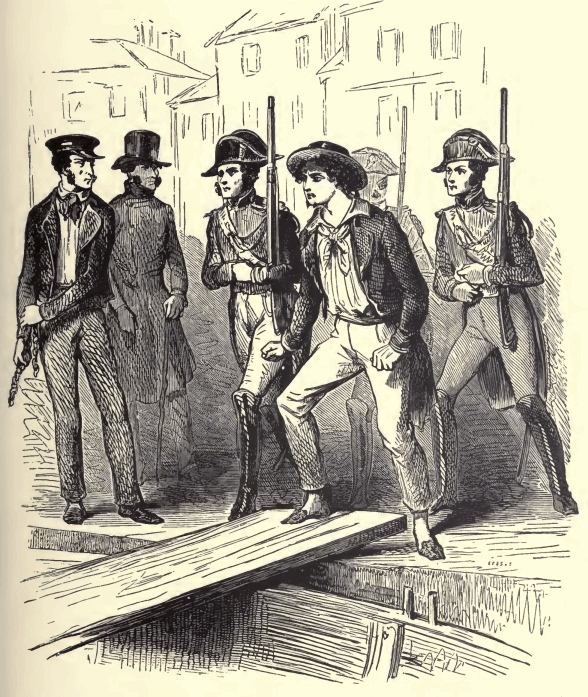
\includegraphics[width=\textwidth]{0111m.jpg}
\end{figure}

The boat continued her voyage. They had passed the Tête de Mort, were
now off the Anse du Pharo, and about to double the battery. This
manœuvre was incomprehensible to Dantès.

“Whither are you taking me?” asked he.

“You will soon know.”

“But still——”

“We are forbidden to give you any explanation.” Dantès, trained in
discipline, knew that nothing would be more absurd than to question
subordinates, who were forbidden to reply; and so he remained silent.

The most vague and wild thoughts passed through his mind. The boat they
were in could not make a long voyage; there was no vessel at anchor
outside the harbor; he thought, perhaps, they were going to leave him
on some distant point. He was not bound, nor had they made any attempt
to handcuff him; this seemed a good augury. Besides, had not the
deputy, who had been so kind to him, told him that provided he did not
pronounce the dreaded name of Noirtier, he had nothing to apprehend?
Had not Villefort in his presence destroyed the fatal letter, the only
proof against him?

He waited silently, striving to pierce through the darkness.

They had left the Ile Ratonneau, where the lighthouse stood, on the
right, and were now opposite the Point des Catalans. It seemed to the
prisoner that he could distinguish a feminine form on the beach, for it
was there Mercédès dwelt. How was it that a presentiment did not warn
Mercédès that her lover was within three hundred yards of her?

One light alone was visible; and Dantès saw that it came from Mercédès’
chamber. Mercédès was the only one awake in the whole settlement. A
loud cry could be heard by her. But pride restrained him and he did not
utter it. What would his guards think if they heard him shout like a
madman?

He remained silent, his eyes fixed upon the light; the boat went on,
but the prisoner thought only of Mercédès. An intervening elevation of
land hid the light. Dantès turned and perceived that they had got out
to sea. While he had been absorbed in thought, they had shipped their
oars and hoisted sail; the boat was now moving with the wind.

In spite of his repugnance to address the guards, Dantès turned to the
nearest gendarme, and taking his hand,

“Comrade,” said he, “I adjure you, as a Christian and a soldier, to
tell me where we are going. I am Captain Dantès, a loyal Frenchman,
thought accused of treason; tell me where you are conducting me, and I
promise you on my honor I will submit to my fate.”

The gendarme looked irresolutely at his companion, who returned for
answer a sign that said, “I see no great harm in telling him now,” and
the gendarme replied:

“You are a native of Marseilles, and a sailor, and yet you do not know
where you are going?”

“On my honor, I have no idea.”

“Have you no idea whatever?”

“None at all.”

“That is impossible.”

“I swear to you it is true. Tell me, I entreat.”

“But my orders.”

“Your orders do not forbid your telling me what I must know in ten
minutes, in half an hour, or an hour. You see I cannot escape, even if
I intended.”

“Unless you are blind, or have never been outside the harbor, you must
know.”

“I do not.”

“Look round you then.” Dantès rose and looked forward, when he saw rise
within a hundred yards of him the black and frowning rock on which
stands the Château d’If. This gloomy fortress, which has for more than
three hundred years furnished food for so many wild legends, seemed to
Dantès like a scaffold to a malefactor.

“The Château d’If?” cried he, “what are we going there for?”

The gendarme smiled.

“I am not going there to be imprisoned,” said Dantès; “it is only used
for political prisoners. I have committed no crime. Are there any
magistrates or judges at the Château d’If?”

“There are only,” said the gendarme, “a governor, a garrison, turnkeys,
and good thick walls. Come, come, do not look so astonished, or you
will make me think you are laughing at me in return for my good
nature.”

Dantès pressed the gendarme’s hand as though he would crush it.

“You think, then,” said he, “that I am taken to the Château d’If to be
imprisoned there?”

“It is probable; but there is no occasion to squeeze so hard.”

“Without any inquiry, without any formality?”

“All the formalities have been gone through; the inquiry is already
made.”

“And so, in spite of M. de Villefort’s promises?”

“I do not know what M. de Villefort promised you,” said the gendarme,
“but I know we are taking you to the Château d’If. But what are you
doing? Help, comrades, help!”

By a rapid movement, which the gendarme’s practiced eye had perceived,
Dantès sprang forward to precipitate himself into the sea; but four
vigorous arms seized him as his feet quitted the bottom of the boat. He
fell back cursing with rage.

“Good!” said the gendarme, placing his knee on his chest; “this is the
way you keep your word as a sailor! Believe soft-spoken gentlemen
again! Hark ye, my friend, I have disobeyed my first order, but I will
not disobey the second; and if you move, I will blow your brains out.”
And he levelled his carbine at Dantès, who felt the muzzle against his
temple.

For a moment the idea of struggling crossed his mind, and of so ending
the unexpected evil that had overtaken him. But he bethought him of M.
de Villefort’s promise; and, besides, death in a boat from the hand of
a gendarme seemed too terrible. He remained motionless, but gnashing
his teeth and wringing his hands with fury.

At this moment the boat came to a landing with a violent shock. One of
the sailors leaped on shore, a cord creaked as it ran through a pulley,
and Dantès guessed they were at the end of the voyage, and that they
were mooring the boat.

His guards, taking him by the arms and coat-collar, forced him to rise,
and dragged him towards the steps that lead to the gate of the
fortress, while the police officer carrying a musket with fixed bayonet
followed behind.

Dantès made no resistance; he was like a man in a dream; he saw
soldiers drawn up on the embankment; he knew vaguely that he was
ascending a flight of steps; he was conscious that he passed through a
door, and that the door closed behind him; but all this indistinctly as
through a mist. He did not even see the ocean, that terrible barrier
against freedom, which the prisoners look upon with utter despair.

They halted for a minute, during which he strove to collect his
thoughts. He looked around; he was in a court surrounded by high walls;
he heard the measured tread of sentinels, and as they passed before the
light he saw the barrels of their muskets shine.

They waited upwards of ten minutes. Certain Dantès could not escape,
the gendarmes released him. They seemed awaiting orders. The orders
came.

“Where is the prisoner?” said a voice.

“Here,” replied the gendarmes.

“Let him follow me; I will take him to his cell.”

“Go!” said the gendarmes, thrusting Dantès forward.

The prisoner followed his guide, who led him into a room almost under
ground, whose bare and reeking walls seemed as though impregnated with
tears; a lamp placed on a stool illumined the apartment faintly, and
showed Dantès the features of his conductor, an under-jailer,
ill-clothed, and of sullen appearance.

\begin{figure}[h]
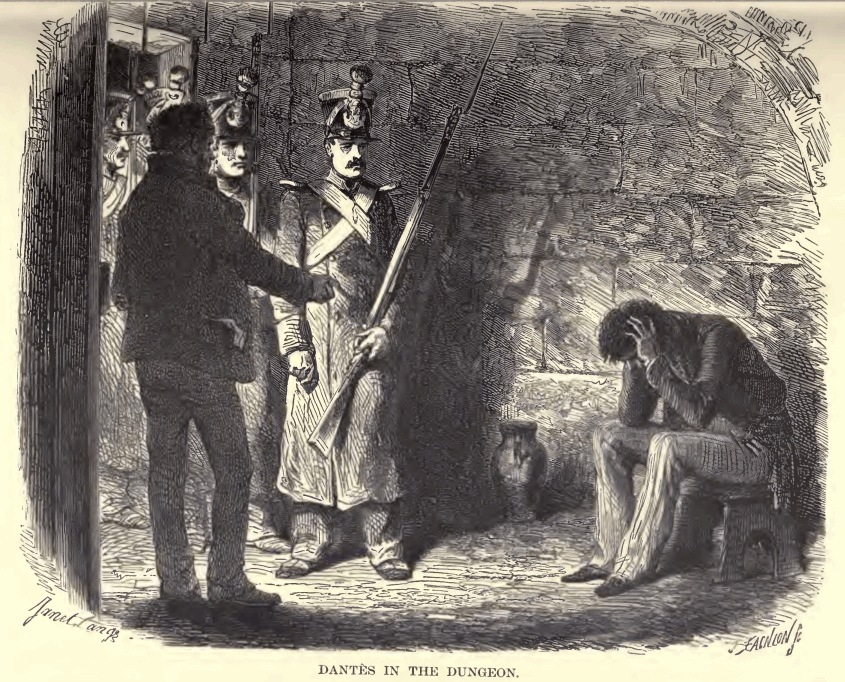
\includegraphics[width=\textwidth]{0113m.jpg}
\end{figure}

“Here is your chamber for tonight,” said he. “It is late, and the
governor is asleep. Tomorrow, perhaps, he may change you. In the
meantime there is bread, water, and fresh straw; and that is all a
prisoner can wish for. Goodnight.” And before Dantès could open his
mouth—before he had noticed where the jailer placed his bread or the
water—before he had glanced towards the corner where the straw was, the
jailer disappeared, taking with him the lamp and closing the door,
leaving stamped upon the prisoner’s mind the dim reflection of the
dripping walls of his dungeon.

Dantès was alone in darkness and in silence—cold as the shadows that he
felt breathe on his burning forehead. With the first dawn of day the
jailer returned, with orders to leave Dantès where he was. He found the
prisoner in the same position, as if fixed there, his eyes swollen with
weeping. He had passed the night standing, and without sleep. The
jailer advanced; Dantès appeared not to perceive him. He touched him on
the shoulder. Edmond started.

“Have you not slept?” said the jailer.

“I do not know,” replied Dantès. The jailer stared.

“Are you hungry?” continued he.

“I do not know.”

“Do you wish for anything?”

“I wish to see the governor.”

The jailer shrugged his shoulders and left the chamber.

Dantès followed him with his eyes, and stretched forth his hands
towards the open door; but the door closed. All his emotion then burst
forth; he cast himself on the ground, weeping bitterly, and asking
himself what crime he had committed that he was thus punished.

The day passed thus; he scarcely tasted food, but walked round and
round the cell like a wild beast in its cage. One thought in particular
tormented him: namely, that during his journey hither he had sat so
still, whereas he might, a dozen times, have plunged into the sea, and,
thanks to his powers of swimming, for which he was famous, have gained
the shore, concealed himself until the arrival of a Genoese or Spanish
vessel, escaped to Spain or Italy, where Mercédès and his father could
have joined him. He had no fears as to how he should live—good seamen
are welcome everywhere. He spoke Italian like a Tuscan, and Spanish
like a Castilian; he would have been free, and happy with Mercédès and
his father, whereas he was now confined in the Château d’If, that
impregnable fortress, ignorant of the future destiny of his father and
Mercédès; and all this because he had trusted to Villefort’s promise.
The thought was maddening, and Dantès threw himself furiously down on
his straw. The next morning at the same hour, the jailer came again.

“Well,” said the jailer, “are you more reasonable today?” Dantès made
no reply.

“Come, cheer up; is there anything that I can do for you?”

“I wish to see the governor.”

“I have already told you it was impossible.”

“Why so?”

“Because it is against prison rules, and prisoners must not even ask
for it.”

“What is allowed, then?”

“Better fare, if you pay for it, books, and leave to walk about.”

“I do not want books, I am satisfied with my food, and do not care to
walk about; but I wish to see the governor.”

“If you worry me by repeating the same thing, I will not bring you any
more to eat.”

“Well, then,” said Edmond, “if you do not, I shall die of hunger—that
is all.”

The jailer saw by his tone he would be happy to die; and as every
prisoner is worth ten sous a day to his jailer, he replied in a more
subdued tone.

“What you ask is impossible; but if you are very well behaved you will
be allowed to walk about, and some day you will meet the governor, and
if he chooses to reply, that is his affair.”

“But,” asked Dantès, “how long shall I have to wait?”

“Ah, a month—six months—a year.”

“It is too long a time. I wish to see him at once.”

“Ah,” said the jailer, “do not always brood over what is impossible, or
you will be mad in a fortnight.”

“You think so?”

“Yes; we have an instance here; it was by always offering a million of
francs to the governor for his liberty that an abbé became mad, who was
in this chamber before you.”

\begin{figure}[h]
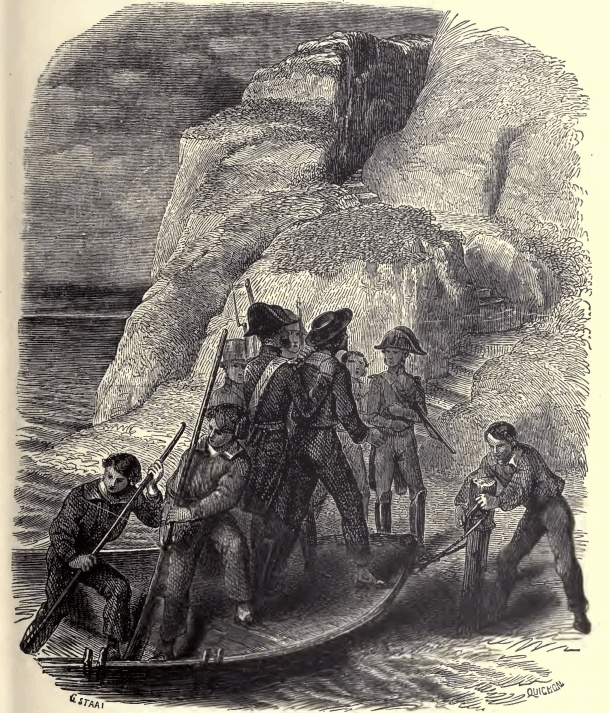
\includegraphics[width=\textwidth]{0119m.jpg}
\end{figure}

“How long has he left it?”

“Two years.”

“Was he liberated, then?”

“No; he was put in a dungeon.”

“Listen!” said Dantès. “I am not an abbé, I am not mad; perhaps I shall
be, but at present, unfortunately, I am not. I will make you another
offer.”

“What is that?”

“I do not offer you a million, because I have it not; but I will give
you a hundred crowns if, the first time you go to Marseilles, you will
seek out a young girl named Mercédès, at the Catalans, and give her two
lines from me.”

\begin{figure}[h]
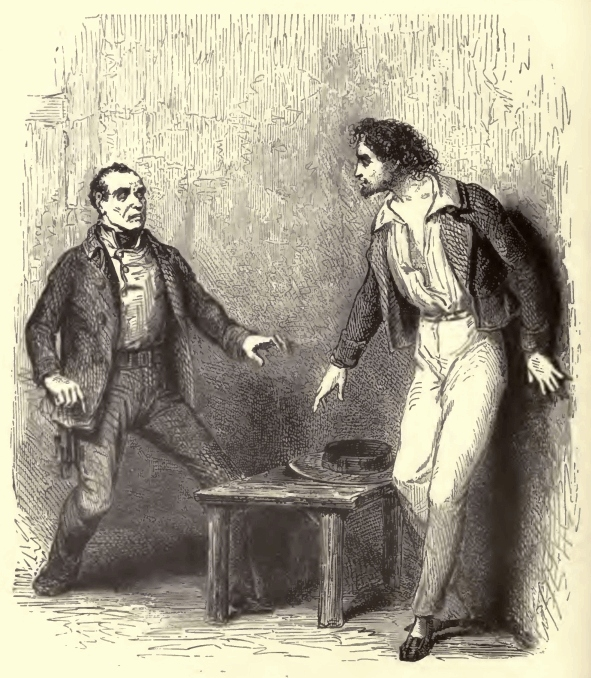
\includegraphics[width=\textwidth]{0120m.jpg}
\end{figure}

“If I took them, and were detected, I should lose my place, which is
worth two thousand francs a year; so that I should be a great fool to
run such a risk for three hundred.”

“Well,” said Dantès, “mark this; if you refuse at least to tell
Mercédès I am here, I will some day hide myself behind the door, and
when you enter I will dash out your brains with this stool.”

“Threats!” cried the jailer, retreating and putting himself on the
defensive; “you are certainly going mad. The abbé began like you, and
in three days you will be like him, mad enough to tie up; but,
fortunately, there are dungeons here.”

Dantès whirled the stool round his head.

“All right, all right,” said the jailer; “all right, since you will
have it so. I will send word to the governor.”

“Very well,” returned Dantès, dropping the stool and sitting on it as
if he were in reality mad. The jailer went out, and returned in an
instant with a corporal and four soldiers.

“By the governor’s orders,” said he, “conduct the prisoner to the tier
beneath.”

“To the dungeon, then,” said the corporal.

“Yes; we must put the madman with the madmen.” The soldiers seized
Dantès, who followed passively.

He descended fifteen steps, and the door of a dungeon was opened, and
he was thrust in. The door closed, and Dantès advanced with
outstretched hands until he touched the wall; he then sat down in the
corner until his eyes became accustomed to the darkness. The jailer was
right; Dantès wanted but little of being utterly mad.
